\chapter{Funktionen}

\begin{inhalt}
  Funktionen und ihre Eigenschaften:
  \begin{itemize}
    \item Definition Funktionsbegriff
    \item Wichtige Funktionen
    \item Eigenschaften (Achsenschnittstellen, Monotonie, Grenzwerte)
    \item Trigonometrische Funktionen
  \end{itemize}
\end{inhalt}

\section{Grundlegende Eigenschaften}

\begin{bla}{Funktion}
  Eine \emph{Funktion} ist etwas, das einer Zahl ($x$) eine andere ($f(x)$) zuordnet. $f(x)=x^2$ ordnet beispielsweise einer Zahl $x$ ihr Quadrat, also $x^2$, zu. \\
  Wir können eine Funktion graphisch veranschaulichen, indem wir sie in ein Koordinatensystem zeichnen.

  \begin{marginfigure}
    \begin{tikzpicture}[
        scale=0.7,
        thick,
        >=stealth',
        dot/.style = {
          draw,
          fill = white,
          circle,
          inner sep = 0pt,
          minimum size = 4pt
        }
      ]
      \coordinate (O) at (0,0);

      \draw[step=1cm,gray!40] (-2.9,-0.9) grid (2.9,2.9);

      % Achsen
      \draw[->] (-3,0) -- (3,0) coordinate[label = {below:$x$}] (xmax);
      \draw[->] (0,-1) -- (0,3) coordinate[label = {right:$f(x)$}] (ymax);

      % Graph
      \draw[domain=-2:2,smooth,variable=\x,red, label={right:$f$}] plot ({\x},{\x*\x});
      \draw (2,3.5) node[red,label= {[red]below:$f$}] {};

      % y-Wert
      \draw (1,1) -- (-0.1, 1) node[label = {left:\footnotesize $f(x_0)$}] {};

      % x-Wert und marker
      \draw (1,1) node[dot] {} -- (1,-0.1) node[label = {below:\footnotesize $x_0$}] {};
    \end{tikzpicture}
    \caption{Graph von $f(x)=x^2$. Für einen $x$-Wert von der $x$-Achse (hier $x_0$) kann sein zugehöriger $f(x)$-Wert (hier $f(x_0)$) abgelesen werden.}
  \end{marginfigure}
  \begin{marginfigure}
    \begin{tcolorbox}[colback=white!95!black,colframe=white!75!black,title=CAS:,arc=0mm]
      \begin{scriptsize}
        \textbf{Calculator}: \hfill \( f(x) := |x| \) \\* \ \\*
        \textbf{Graph}: \hfill \( f1(x) = f(x) \)
      \end{scriptsize}
    \end{tcolorbox}
  \end{marginfigure}
\end{bla}

\begin{bla}{Punkt, Stelle, Wert}
  \begin{itemize}
    \item \textbf{Punkt}: Ein Punkt ist ein Zahlenpaar, bestehend aus $x$- und $y$-Wert.
    \item \textbf{Stelle, Wert}: An der \emph{Stelle} $x_0$ hat $f$ den \emph{Wert} $f(x_0)$. Das ergibt den \emph{Punkt} $\mathrm{P}(x_0|f(x_0))$.
  \end{itemize}
\end{bla}

\begin{bla}{Wichtige Funktionen: Betragsfunktion}
  \begin{marginfigure}
    \begin{tikzpicture}[
        scale=0.7,
        thick,
        >=stealth',
        dot/.style = {
          draw,
          fill = white,
          circle,
          inner sep = 0pt,
          minimum size = 4pt
        }
      ]
      \coordinate (O) at (0,0);

      \draw[step=1cm,gray!40] (-2.9,-0.1) grid (2.9,2.9);

      % Achsen
      \draw[->] (-3,0) -- (3,0) coordinate[label = {below:$x$}] (xmax);
      \draw[->] (0,-0.1) -- (0,3) coordinate[label = {right:$f(x)$}] (ymax);

      % Graph
      \draw[domain=-2:0,smooth,variable=\x,red, label={right:$f$}] plot ({\x},{-\x});
      \draw[domain=0:2,smooth,variable=\x,red, label={right:$f$}] plot ({\x},{\x});

      \draw (2,2.8) node[red,label= {[red]below:$|x|$}] {};
    \end{tikzpicture}
    \caption{Graph von $f(x)=|x|$.}
  \end{marginfigure}

  Der \emph{Betrag} $f(x)=|x|$ einer Zahl ist der Abstand der Zahl zum Ursprung auf der Zahlengeraden. Der Betrag hebt also quasi ein $-$ als Vorzeichen auf: $|-5|=5, |3|=3$. Formal gilt:
  \begin{align*}
    |x|=\begin{cases}
        x\  & \text{falls $x\geq 0$} \\
        -x\  & \text{falls $x<0$}
    \end{cases}
  \end{align*}
  Dabei wird ausgenutzt, dass $-(-x)=x$ gilt.
\end{bla}

\clearpage
\begin{bla}{Wichtige Funktionen: Potenzen von $x$}
  Die wohl am häufigsten verwendeten Funktionen sind die \emph{Potenzen} von $x$, also $x^2, x^3$ und so weiter. Sie lassen sich in zwei Sorten unterteilen:
  \begin{itemize}
    \item \textbf{Exponent gerade}: Ist der Exponent gerade, so ist der Graph eine nach oben offene Parabel, die die Achsen im Nullpunkt berührt:

    \begin{marginfigure}[-10em]
      \begin{tikzpicture}[
          scale=0.7,
          thick,
          >=stealth',
          dot/.style = {
            draw,
            fill = white,
            circle,
            inner sep = 0pt,
            minimum size = 4pt
          }
        ]
        \coordinate (O) at (0,0);

        \draw[step=1cm,gray!40] (-2.9,-0.1) grid (2.9,2.9);

        % Achsen
        \draw[->] (-3,0) -- (3,0) coordinate[label = {below:$x$}] (xmax);
        \draw[->] (0,-0.1) -- (0,3) coordinate[label = {right:$f(x)$}] (ymax);

        % Graphen
        \draw[domain=-2:2,smooth,variable=\x,red, label={right:$f$}] plot ({\x},{abs(\x)^2});
        \draw[domain=-1.4:1.4,smooth,variable=\x,blue, label={right:$f$}] plot ({\x},{abs(\x)^4});
        \draw[domain=-1.25:1.25,smooth,variable=\x,orange, label={right:$f$}] plot ({\x},{abs(\x)^6});

        % Marker
        \foreach \foo in {-2,-1,...,2} {
          \draw (\foo,0.1) -- (\foo,-0.1) node[label={below:\foo}] {};
        }
        \foreach \foo in {1,2} {
          \draw (0.1,\foo) -- (-0.1,\foo) node[label={left:\foo}] {};
        }
      \end{tikzpicture}
      \caption{Graph von \textcolor{red}{$x^2$}, \textcolor{blue}{$x^4$} und \textcolor{orange}{$x^6$}.}
    \end{marginfigure}

    \item \textbf{Exponent ungerade}: Ist der Exponent ungerade, so sieht der Graph wie bei einem geraden Exponenten aus, nur, dass die beiden \glqq Äste\grqq des Graphen in unterschiedliche Richtungen zeigen:
    \begin{marginfigure}
      \begin{tikzpicture}[
          scale=0.7,
          thick,
          >=stealth',
          dot/.style = {
            draw,
            fill = white,
            circle,
            inner sep = 0pt,
            minimum size = 4pt
          }
        ]
        \coordinate (O) at (0,0);

        \draw[step=1cm,gray!40] (-2.9,-0.9) grid (2.9,2.9);

        % Achsen
        \draw[->] (-3,0) -- (3,0) coordinate[label = {below:$x$}] (xmax);
        \draw[->] (0,-1) -- (0,3) coordinate[label = {right:$f(x)$}] (ymax);

        % Graphen
        \draw[domain=-1.1:2,smooth,variable=\x,red, label={right:$f$}] plot ({\x},{\x});
        \draw[domain=-1.1:1.4,smooth,variable=\x,blue, label={right:$f$}] plot ({\x},{\x^3});
        \draw[domain=-1.1:1.25,smooth,variable=\x,orange, label={right:$f$}] plot ({\x},{(\x^5});

        % Marker
        \foreach \foo in {-2,-1,...,2} {
          \draw (\foo,0.1) -- (\foo,-0.1) node[label={below:\foo}] {};
        }
        \foreach \foo in {1,2} {
          \draw (0.1,\foo) -- (-0.1,\foo) node[label={left:\foo}] {};
        }
      \end{tikzpicture}
      \caption{Graph von \textcolor{red}{$x$}, \textcolor{blue}{$x^3$} und \textcolor{orange}{$x^5$}.}
    \end{marginfigure}
  \end{itemize}
\end{bla}

\begin{bla}{Grad}
  Ist ein Funktionsterm gegeben, in dem Potenzen von $x$ vorkommen, so ist der \emph{Grad} der Funktion die höchste Potenz von $x$ (bei $f(x)=x^2-3x^3$ wäre der Grad zum Beispiel $3$).
\end{bla}

\begin{bla}{Wichtige Funktionen: Wurzelfunktion}
  \begin{marginfigure}
    \begin{tikzpicture}[
        scale=0.7,
        thick,
        >=stealth',
        dot/.style = {
          draw,
          fill = white,
          circle,
          inner sep = 0pt,
          minimum size = 4pt
        }
      ]
      \coordinate (O) at (0,0);

      \draw[step=1cm,gray!40] (-2.9,-2.9) grid (2.9,2.9);

      % Achsen
      \draw[->] (-3,0) -- (3,0) coordinate[label = {below:$x$}] (xmax);
      \draw[->] (0,-3) -- (0,3) coordinate[label = {right:$f(x)$}] (ymax);

      % Graphen
      \draw[domain=-2:2,smooth,variable=\x,black!60!green, label={right:$f$}] plot ({\x},{abs(\x)^2});
      \draw[domain=0:3,smooth,variable=\x,red, label={right:$f$}] plot ({\x},{sqrt(\x)});
      \draw[domain=0:3,smooth,variable=\x,red!60,dotted, label={right:$f$}] plot ({\x},{-sqrt(\x)});

      % Spiegelung
      \draw[gray, dashed] (-1.5,-1.5) -- (2.5,2.5) node[label={right:Spiegelung}] {};

      \draw (2.3,3.5) node[label= {[black!60!green]below:$x^2$}] {};
      \draw (2.3,1.5) node[label={[red]below:$\sqrt{x}$}] {};
    \end{tikzpicture}
    \caption{Graph von \textcolor{black!60!green}{$x^2$} und \textcolor{red}{$\sqrt{x}$}. Es ist z.B. $-\sqrt{3}*-\sqrt{3}=\sqrt{3}*\sqrt{3}$, deswegen hat jede Zahl eigentlich zwei Wurzeln, aber es wird normalerweise nur die positive Wurzel betrachtet.}
  \end{marginfigure}
  Die \emph{Wurzel} einer Zahl $x$ ist die Zahl, die mit sich selbst multipliziert wieder $x$ ergibt. Wir nennen sie die Wurzel aus $x$, schreibe $\sqrt{x}$:
  \begin{equation*}
    x=\sqrt{x}*\sqrt{x}
  \end{equation*}
  Die Wurzel einer Zahl ist das Gegenteil des \emph{Quadrats} einer Zahl.
\end{bla}

\begin{bla}{Funktionen mit rationalem Exponenten}
  Es ist $\sqrt{x}=x^{\frac{1}{2}}$, weil $x^{\frac{1}{2}}*x^{\frac{1}{2}}=x^{\frac{1}{2}+\frac{1}{2}}=x^1=x$. Allgemein gilt:
  \begin{equation*}
    x^{\frac{p}{q}}=\sqrt[\leftroot{-2}\uproot{2}q]{x^p}
  \end{equation*}
  Muss man eine Wurzelfunktion ableiten, so ist es geschickter, die Funktion als Potenzfunktion zu schreiben.
\end{bla}

\begin{bla}{Punkt auf Funktionsgraphen}
  \begin{marginfigure}
    \begin{tcolorbox}[colback=white!95!black,colframe=white!75!black,title=CAS:,arc=0mm]
      \begin{scriptsize}
        \textbf{Calculator}: \hfill \( f(x) := x^2 \) \\*
        \hfill \( \bm{f(4) \leadsto 16} \)
      \end{scriptsize}
    \end{tcolorbox}
  \end{marginfigure}
  Ist ein Punkt und eine Funktion gegeben, so kann man testen, ob der Punkt auf dem Funktionsgraphen liegt. Liegt der Punkt auf dem Funktionsgraphen, so muss die Funktion für den $x$-Wert des Punktes denselben $y$-Wert haben wie der Punkt. Ist also der Punkt $P(3|1)$ gegeben und die Funktion $f(x)={(x-2)}^2$, so bestimmt man $f(3)$. Es muss $f(3)=1$ gelten.
  \begin{equation*}
    f(3)={(3-2)}^2=1^2=1
  \end{equation*}
  Also liegt der Punkt auf der Geraden.

  \begin{marginfigure}
    \begin{tikzpicture}[
        scale=0.7,
        thick,
        >=stealth',
        dot/.style = {
          draw,
          fill = white,
          circle,
          inner sep = 0pt,
          minimum size = 4pt
        }
      ]
      \coordinate (O) at (0,0);

      \draw[step=1cm,gray!40] (-0.9,-0.9) grid (4.9,4.9);

      % Achsen
      \draw[->] (-1,0) -- (5,0) coordinate[label = {below:$x$}] (xmax);
      \draw[->] (0,-1) -- (0,5) coordinate[label = {right:$f(x)$}] (ymax);

      % Graph
      \draw[domain=-0.1:3.5,smooth,variable=\x,red] plot ({\x},{(\x-2)^2});
      \draw (4.5,3.2) node[red,label= {[red]below:$f(x)={(x-2)}^2$}] {};
      \draw (3,1) node[dot,rotate=45, label={below:$P(3|1)$}] {};

    \end{tikzpicture}
    \caption{Der Graph von $f(x)={(x-2)}^2$ und $P(3|1)$}
  \end{marginfigure}
\end{bla}

\newpage

\begin{bla}{Schnitte von Funktionen}
  \begin{marginfigure}
    \begin{tcolorbox}[colback=white!95!black,colframe=white!75!black,title=CAS:,arc=0mm]
      \begin{scriptsize}
        \textbf{Graph} (\( f1(x) = \ \sim \), \( f2(x) = \ \sim \)): \\*
        \menu{Menü > Graph anal. > Schnittpunkte} \\*
        \( \leadsto \) Bereich auswählen (mit genau \\* \text{\phantom{\( \leadsto \)}} einem Schnitt drin) \\*
        \( \leadsto \) Werte ablesen
      \end{scriptsize}
    \end{tcolorbox}
  \end{marginfigure}
  Zwei Funktionen schneiden sich dort, wo sie für einen $x$-Wert den gleichen $y$-Wert haben. Man bestimmt diese Punkte, indem man die beiden Funktionen gleichsetzt.
\end{bla}

\begin{koch}
  \begin{enumerate}
    \item Funktionen gleichsetzen $\Rightarrow$ $x$-Werte
    \item $x$-Werte in eine der Funktionen einsetzen $\Rightarrow$ $y$-Werte
    \item Die Schnittpunkte der Funktionen sind die $x$-Werte mit ihren zugehörigen $y$-Werten.
  \end{enumerate}
\end{koch}



\section{Kurvendiskussion}

\begin{bla}{Achsenschnittstellen}
  \begin{marginfigure}[8em]
    \begin{tikzpicture}[
        scale=0.7,
        thick,
        >=stealth',
        dot/.style = {
          draw,
          fill = white,
          circle,
          inner sep = 0pt,
          minimum size = 4pt
        }
      ]
      \coordinate (O) at (0,0);

      \draw[step=1cm,gray!40] (-2.9,-2.9) grid (2.9,2.9);

      % Achsen
      \draw[->] (-3,0) -- (3,0) coordinate[label = {below:$x$}] (xmax);
      \draw[->] (0,-3) -- (0,3) coordinate[label = {right:$f(x)$}] (ymax);

      % Graph
      \draw[domain=-0.8:1.3,smooth,variable=\x,red, label={right:$f$}] plot ({\x},{(\x-0.5)^3+1});
      \draw (2,1.5) node[red,label= {[red]below:$(x-\frac{1}{2})^3+1$}] {};

      % Nullstelle
      \draw (-0.5,0) node[dot] {};

      % y-Achsenabschnitt
      \draw (0,0.875) node[dot] {};
    \end{tikzpicture}
    \caption{Der Graph von $f(x)={(x-\frac{1}{2})}^3+1$ und seine Achsenschnittstellen}
  \end{marginfigure}
  \begin{marginfigure}
    \begin{tcolorbox}[colback=white!95!black,colframe=white!75!black,title=CAS:,arc=0mm]
      \begin{scriptsize}
        \textbf{Calculator}: \\*
        Schnitt \( y \)-Achse: \hfill \( f(0) \) \\*
        Schnitte \( x \)-Achse: \hfill \textsc{zeros}\( (f(x), x) \) \\* \ \\*
        \textbf{Graph} (\( f1(x) = \ \sim \)): \\*
        \menu{Menü > Graph anal > Nullstellen} \\*
        \( \to \) Bereich mit genau einer Nullstelle \\* \( \text{\phantom{\( \leadsto \)}} \) auswählen
      \end{scriptsize}
    \end{tcolorbox}
  \end{marginfigure}
  Am leichtesten zu untersuchen sind wohl die \emph{Achsenschnittstellen} einer Funktion. Dabei unterscheidet man logischerweise zwischen der $x$-Achse (Nullstellen) und der $y$-Achse ($y$-Achsenabschnitt).
  \begin{itemize}
    \item \textbf{Nullstellen}: Nullstellen sind die $x$-Werte, für die $f(x)=0$ gilt. Lösungsansätze hierfür sind beispielsweise die \textbf{Mitternachtsformel} oder der \textbf{Satz vom Nullprodukt}.
    \item \textbf{y-Achsenabschnitt}: Der y-Achsenabschnitt einer Funktion ist der Funktionswert für $x=0$, also $f(0)$.
  \end{itemize}
\end{bla}

\begin{bla}{Monotonie}
  \begin{marginfigure}
    \begin{tikzpicture}[
        thick,
        >=stealth',
        dot/.style = {
          draw,
          fill = white,
          circle,
          inner sep = 0pt,
          minimum size = 4pt
        }
      ]
      \coordinate (O) at (0,0);

      \draw[step=1cm,gray!40] (-0.9,-0.9) grid (2.9,2.9);

      % Achsen
      \draw[->] (-1,0) -- (3,0) coordinate[label = {below:$x$}] (xmax);
      \draw[->] (0,-1) -- (0,3) coordinate[label = {right:$f(x)$}] (ymax);

      % streng monoton fallend
      \draw[domain=0:1.5,smooth,variable=\x,red] plot ({\x},{-\x*\x+2});

      % monoton fallend TODO falsche Funktion!
      \draw[domain=0:2.05,smooth,variable=\x,orange] plot ({\x},{-(\x-1)^3+1});

      % monoton steigend TODO falsche Funktion!
      \draw[domain=0:2.05,smooth,variable=\x,black!60!green] plot ({\x},{(\x-1)^3+1});

      % streng monoton steigend
      \draw[domain=0:1.5,smooth,variable=\x,blue] plot ({\x},{\x*\x});

    \end{tikzpicture}
    \caption{\textcolor{red}{Streng monoton fallende}, \textcolor{orange}{monoton fallende}, \textcolor{black!60!green}{monoton wachsende} und \textcolor{blue}{streng monoton wachsende} Funktion.}
  \end{marginfigure}
  Unter dem Begriff \emph{Monotonie} versteht man die Untersuchung des Krümmungsverhaltens einer Funktion $f(x)$ auf einem Intervall $[a,b]$. Man unterscheidet dabei vier verschiedene Monotonietypen:
  \begin{itemize}
    \item \textbf{Streng monoton fallend}: $f(x)$ ist auf $[a,b]$ streng monoton fallend, wenn für zwei verschiedene Werte $x,y$ auf $[a,b]$ mit $x<y$ stets gilt: $f(x)>f(y)$.
    \item \textbf{Monoton fallend}: $f(x)$ ist auf $[a,b]$ monoton fallend, wenn für zwei verschiedene Werte $x,y$ auf $[a,b]$ mit $x<y$ stets gilt: $f(x)\geq f(y)$.
    \item \textbf{Monoton wachsend}: $f(x)$ ist auf $[a,b]$ monoton wachsend, wenn für zwei verschiedene Werte $x,y$ auf $[a,b]$ mit $x<y$ stets gilt: $f(x)\leq f(y)$.
    \item \textbf{Streng monoton wachsend}: $f(x)$ ist auf $[a,b]$ streng monoton wachsend, wenn für zwei verschiedene Werte $x,y$ auf $[a,b]$ mit $x<y$ stets gilt: $f(x)<f(y)$.
  \end{itemize}
\end{bla}

\clearpage
\begin{bla}{Verhalten für $x\rightarrow \pm \infty$}
  \begin{marginfigure}
    \begin{tcolorbox}[colback=white!95!black,colframe=white!75!black,title=CAS:,arc=0mm]
      \begin{scriptsize}
        \textbf{Calculator}: \\*
        Sonderzeichen \( \to \) lim \\*
        \hfill \( \lim_{x \to \infty} {\left( 1- \tfrac{1}{x} \right)}^x \) \\*
        (man erhält die \( \infty \) über \( \pi \blacktriangleright \))
      \end{scriptsize}
    \end{tcolorbox}
  \end{marginfigure}
  \begin{marginfigure}
      \begin{tikzpicture}[
          thick,
          >=stealth',
          dot/.style = {
            draw,
            fill = white,
            circle,
            inner sep = 0pt,
            minimum size = 4pt
          }
        ]
        \coordinate (O) at (0,0);

        \draw[step=1cm,gray!40] (-0.9,-0.9) grid (2.9,2.9);

        % Achsen
        \draw[->] (-1,0) -- (3,0) coordinate[label = {below:$x$}] (xmax);
        \draw[->] (0,-1) -- (0,3) coordinate[label = {right:$f(x)$}] (ymax);

        % streng monoton fallend
        \draw[domain=-0.3:2.9,smooth,variable=\x,red] plot ({\x},{exp(-\x)});
      \end{tikzpicture}
      \caption{$f(x)=e^{-x}$ geht für $x\rightarrow\infty$ gegen $0$.}
    \end{marginfigure}
  Es gibt zwei Möglichkeiten, wie sich eine Funktion für $x$ gegen $\pm \infty$ verhalten kann:
  \begin{itemize}
    \item Der Funktionswert geht gegen $\pm \infty$.
    \item Der Funktionswert geht gegen einen festen Wert, meistens $0$.
  \end{itemize}
  Dabei gilt es zu beachten, dass Potenzen von $x$ schneller gegen $\pm \infty$ gehen, je größer der Exponent ist. Steht $x$ im Exponenten, so geht der Funktionswert schneller gegen $\pm \infty$ als jede Potenz von $x$. Das bedeutet konkret, dass beispielsweise $x^{1000}*e^{-x}$ für $x \rightarrow \infty$ gegen $0$ geht, da $e^{-x}$ für große $x$ `stärker' gegen $0$ geht als $x^{1000}$ gegen $\infty$, obwohl es, wenn man die beiden Graphen zeichnet, erst nicht so aussieht.
\end{bla}



\begin{bla}{Asymptoten}
  \begin{itemize}
    \item \textbf{waagerechte Asymptote}: Geht die Funktion für $x \rightarrow \infty$ gegen einen festen Wert, so hat sie eine \emph{waagerechte} Asymptote ($f(x)=e^{-x}$ geht gegen $0$).
    \item \textbf{schiefe Asymptote}: Besteht die Funktion aus mehreren Summanden, so können wir für $x \rightarrow \infty$ diejenigen mit einer waagerechten Asymptote durch ihre Asymptote ersetzen, es entsteht eine schiefe Asymptote ($f(x)=2x+e^{-x}$ geht gegen $2x$).
  \end{itemize}
\end{bla}

\begin{bla}{Kurven verschieben}
	\begin{enumerate}
    \item \textbf{Verschieben nach rechts/links}: Verschieben um $3$ nach links: $x$ durch $(x+3)$ ersetzen (nach rechts: $x$ durch $(x-3)$ ersetzen). Die Klammern dürfen nicht vergessen werden!

    \item \textbf{Verschieben nach oben/unten}: Verschieben um $3$ nach oben: $+3$ an den Funktionsterm anhängen (nach unten: $-3$ an den Funktionsterm anhängen).
  \end{enumerate}
\begin{marginfigure}
  \begin{tikzpicture}[
      scale=0.7,
      thick,
      >=stealth',
      dot/.style = {
        draw,
        fill = white,
        circle,
        inner sep = 0pt,
        minimum size = 4pt
      }
    ]
    \coordinate (O) at (0,0);

    \draw[step=1cm,gray!40] (-2.9,-0.1) grid (2.9,2.9);

    % Achsen
    \draw[->] (-3,0) -- (3,0) coordinate[label = {below:$x$}] (xmax);
    \draw[->] (0,-0.1) -- (0,3) coordinate[label = {right:$f(x)$}] (ymax);

    % Graph
    \draw[domain=-1.5:1.5,smooth,variable=\x,red, label={right:$f$}] plot ({\x},{(\x)^2});
    \draw[domain=-0.5:2.5,smooth,variable=\x,black!60!green, label={right:$f$}] plot ({\x},{(\x-1)^2});
  \end{tikzpicture}
  \caption{\textcolor{red}{$f(x)=x^2$} und \textcolor{black!60!green}{$f(x)={(x-1)}^2$}.}
\end{marginfigure}

\begin{marginfigure}
  \begin{tikzpicture}[
      scale=0.7,
      thick,
      >=stealth',
      dot/.style = {
        draw,
        fill = white,
        circle,
        inner sep = 0pt,
        minimum size = 4pt
      }
    ]
    \coordinate (O) at (0,0);

    \draw[step=1cm,gray!40] (-2.9,-0.1) grid (2.9,2.9);

    % Achsen
    \draw[->] (-3,0) -- (3,0) coordinate[label = {below:$x$}] (xmax);
    \draw[->] (0,-0.1) -- (0,3) coordinate[label = {right:$f(x)$}] (ymax);

    % Graph
    \draw[domain=-1.5:1.5,smooth,variable=\x,red, label={right:$f$}] plot ({\x},{(\x)^2});
    \draw[domain=-1.5:1.5,smooth,variable=\x,black!60!green, label={right:$f$}] plot ({\x},{(\x)^2+1});
  \end{tikzpicture}
  \caption{\textcolor{red}{$f(x)=x^2$} und \textcolor{black!60!green}{$f(x)=x^2+1$}.}
\end{marginfigure}

\begin{bla}{Kurven strecken/stauchen oder an der $x$-Achse spiegeln}
  \begin{enumerate}
    \item \textbf{Strecken}: um den Faktor 3: Funktionsterm mit $3$ multiplizieren.
    \item \textbf{Stauchen}: um den Faktor 3: Funktionsterm mit $\tfrac{1}{3}$ multiplizieren.
    \item \textbf{Spiegeln}: Funktionsterm mit $(-1)$ multiplizieren.
  \end{enumerate}
  \textbf{Achtung}: Man muss den \emph{ganzen} Funktionsterm mit dem jeweiligen Faktor multiplizieren, deswegen ist es sinnvoll, erst Klammern um den ganzen Funktionsterm zu setzen, damit man keine Fehler macht.
\end{bla}

\begin{marginfigure}
  \begin{tikzpicture}[
      scale=0.7,
      thick,
      >=stealth',
      dot/.style = {
        draw,
        fill = white,
        circle,
        inner sep = 0pt,
        minimum size = 4pt
      }
    ]
    \coordinate (O) at (0,0);

    \draw[step=1cm,gray!40] (-2.9,-0.1) grid (2.9,2.9);

    % Achsen
    \draw[->] (-3,0) -- (3,0) coordinate[label = {below:$x$}] (xmax);
    \draw[->] (0,-0.1) -- (0,3) coordinate[label = {right:$f(x)$}] (ymax);

    % Graph
    \draw[domain=-1.5:1.5,smooth,variable=\x,red, label={right:$f$}] plot ({\x},{(\x)^2});
    \draw[domain=-2:2,smooth,variable=\x,black!60!green, label={right:$f$}] plot ({\x},{0.5*(\x)^2});
    \draw[domain=-1.2:1.2,smooth,variable=\x,blue, label={right:$f$}] plot ({\x},{2*(\x)^2});
  \end{tikzpicture}
  \caption{\textcolor{red}{$f(x)=x^2$}, \textcolor{black!60!green}{$f(x)=\frac{1}{2} x^2$} und \textcolor{blue}{$f(x)=2x^2$}.}
\end{marginfigure}
\end{bla}

\begin{bla}{Mehrere Transformationen}
  Natürlich kann man eine Funktion auch mehrmals transformieren, also zum Beispiel nach $(2|1)$ verschieben (also $2$ nach rechts und $1$ nach oben) dann spiegeln und dann schließlich um den Faktor $2$ strecken. Durch diese Hintereinanderausführung von Transformationen kann man sehr viele verschiedene Funktionsgraphen erzeugen.
\end{bla}

\begin{koch}
  \textbf{Erkennen von Funktionen} \\
  Gegeben: Graph. Gesucht: Funktion des Graphen.
  \begin{enumerate}
    \item \textbf{Grundlegende Funktion}: Welche Funktion könnte zugrunde liegen? Häufig kommen $x^2$, $x^3$, $\sin(x)$ und $e^x$ vor.
    \item \textbf{Strecken/Stauchen}:
      \begin{itemize}
        \item \textbf{Potenz von $x$} ($x^2$,$x^3$,\dots): Würde man den Graphen zum Ursprung verschieben, welchen Wert hätte er dann für $x=1$? Ungestreckt/-gestaucht wäre er $1$ (da $1^1=1^2=1$). Ist er zum Beispiel $f(1)=\frac{1}{4}$, so muss der Funktionsterm mit $\frac{1}{4}$ multipliziert werden.
        \item \textbf{Sinuskurve}: Würde man den Graphen zum Ursprung verschieben, was wäre sein größter Abstand zur $x$-Achse? Für $\sin(x)$ ist das normalerweise $1$. Ermittle den Faktor für den Funktionsterm wie bei einer Potenz von $x$.
        \item \textbf{Exponentialfunktion}: Würde man den Graphen zum Ursprung verschieben (also so, dass er für immer kleiner werdende $x$ von oben gegen $-\infty$ gehen würde), wo würde er die $y$-Achse schneiden? Normalerweise wäre das bei $f(0)=e^0=1$. Ermittle den Faktor für den Funktionsterm wie bei einer Potenz von $x$.
      \end{itemize}
    \item \textbf{An die richtige Stelle verschieben}: Bestimme die Koordinaten des Punktes, der normalerweise am Koordinatenursprung liegt und verschiebe die Funktion dorthin.
    \item \textbf{Spiegeln}: Gegebenenfalls muss man den Funktionsterm noch mit $(-1)$ multiplizieren.
  \end{enumerate}
\end{koch}

\clearpage

\section{Trigonometrie}
\begin{marginfigure}
  \begin{tcolorbox}[colback=white!95!black,colframe=white!75!black,title=CAS:,arc=0mm]
    \begin{scriptsize}
      \textbf{Achtung!} Bogenmaß einstellen! \\*
      Auf dem aktuellen Dokument: Dok \( \blacktriangledown \) \( \to \) Einstellungen \( \to \) Dokumenteinstellungen \( \to \) Winkel
    \end{scriptsize}
  \end{tcolorbox}
\end{marginfigure}
Die Grundlage der Trigonometrie sind die Untersuchungen der Verhältnisse von Winkeln und Seitenlängen im rechtwinkligen Dreieck.

\begin{bla}{Bezeichnungen im Dreieck}
  \begin{marginfigure}
    \begin{tikzpicture}[
        thick,
        >=stealth',
        dot/.style = {
          draw,
          fill = white,
          circle,
          inner sep = 0pt,
          minimum size = 4pt
        }
      ]
      \coordinate (O) at (0,0);

      % Dreieck
      \filldraw[draw=red,fill=red!20] (0,0) -- (3,0) -- (3,2) -- cycle;
      \filldraw[fill=green!20,draw=green!50!black] (0,0) -- (0.8,0)
        arc [start angle=0, end angle=33.9, radius=0.8] -- cycle;

      % Labels
      \draw (0.5,-0.1) node[label={[green!50!black]$\alpha$}] {};
      \draw (3,1) node[label={[red]right:Gegenkathete}] {};
      \draw (1.5,1.2) node[label={[red]left:Hypothenuse}] {};
      \draw (1.5,0) node[label={[red]below:Ankathete}] {};

    \end{tikzpicture}
    \caption{Ein rechtwinkliges Dreieck und die Seitenbezeichnungen für den betrachteten Winkel.}
  \end{marginfigure}

  Betrachtet man einen Winkel $\alpha$ in einem rechtwinkligen Dreieck (das heißt, dass ein Innenwinkel des Dreiecks $90^{\circ}$ beträgt), so ergeben sich folgende Namen für die Seiten:
  \begin{itemize}
    \item \textbf{Gegenkathete}: Das ist die dem Winkel gegenüberliegende Seite, also die Seite, die den Winkel nicht berührt.
    \item \textbf{Hypotenuse}: Das ist diejenige der den Winkel berührenden Seiten, die die  längste im Dreieck ist. Sie liegt dem rechten Winkel gegenüber.
    \item \textbf{Ankathete}: Das ist die Seite, die den Winkel berührt, aber nicht die Hypotenuse ist.
  \end{itemize}
\end{bla}

\begin{bla}{Sinus und Cosinus}
  Sinus und Cosinus sind zwei Werte, die das Verhältnis zwischen den Seiten in einem Dreieck darstellen. Sie hängen dabei lediglich vom Winkel zwischen der Ankathete und der Hypotenuse ab (siehe letzte Grafik).
  \begin{enumerate}
    \item \textbf{Sinus}: Der Sinus ist das Verhältnis von Gegenkathete zur Hypotenuse: $\sin \alpha = \frac{\text{Gegenkathete}}{\text{Hypotenuse}}$.
    \item \textbf{Cosinus}: Der Cosinus ist das Verhältnis von Ankathete zur Hypotenuse: $\cos \alpha = \frac{\text{Ankathete}}{\text{Hypotenuse}}$.
  \end{enumerate}
\end{bla}

\begin{bla}{Der Einheitskreis}
  Der \emph{Einheitskreis} ist ein Kreis um den Ursprung des Koordinatensystems mit dem Radius $1$. Er wird benutzt, um die Verhältnisse der Seiten in einem Dreieck zu veranschaulichen, da die Hypotenuse stets die Länge $1$ hat (sie ist der Radius). \\
  Daraus ergibt sich für Sinus und Cosinus in diesem Dreieck: \\
  \begin{itemize}
    \item $\sin \alpha = \frac{\text{Gegenkathete}}{\text{Hypotenuse}} = \frac{\text{Gegenkathete}}{1} = \text{Gegenkathete}$
    \item $\cos \alpha = \frac{\text{Ankathete}}{\text{Hypotenuse}} = \frac{\text{Ankathete}}{1} = \text{Ankathete}$
  \end{itemize}

\begin{marginfigure}
  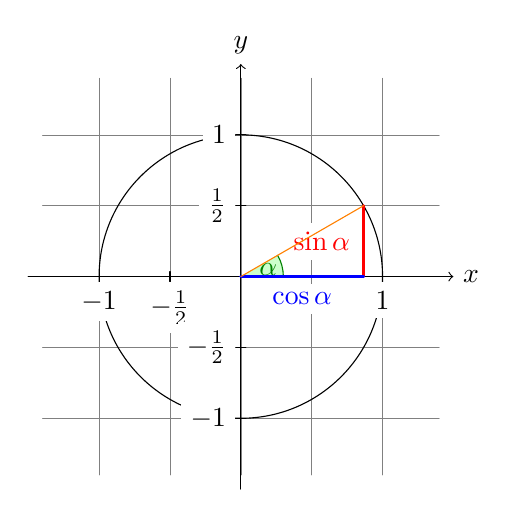
\begin{tikzpicture}
    [scale=1.8,line cap=round,
    % Styles
    axes/.style=,
    important line/.style={very thick},
    information text/.style={rounded corners,fill=red!10,inner sep=1ex}]
    % Colors
    \colorlet{anglecolor}{green!50!black}
    \colorlet{sincolor}{red}
    \colorlet{tancolor}{orange!80!black}
    \colorlet{coscolor}{blue}
    % The graphic
    \draw[help lines,step=0.5cm] (-1.4,-1.4) grid (1.4,1.4);
    \draw (0,0) circle [radius=1cm];
    \begin{scope}[axes]
      \draw[->] (-1.5,0) -- (1.5,0) node[right] {$x$} coordinate(x axis);
      \draw[->] (0,-1.5) -- (0,1.5) node[above] {$y$} coordinate(y axis);
      \foreach \x/\xtext in {-1, -.5/-\frac{1}{2}, 1}
      \draw[xshift=\x cm] (0pt,1pt) -- (0pt,-1pt) node[below,fill=white] {$\xtext$};
      \foreach \y/\ytext in {-1, -.5/-\frac{1}{2}, .5/\frac{1}{2}, 1}
      \draw[yshift=\y cm] (1pt,0pt) -- (-1pt,0pt) node[left,fill=white] {$\ytext$};
    \end{scope}
    \filldraw[fill=green!20,draw=anglecolor] (0,0) -- (3mm,0pt)
    arc [start angle=0, end angle=30, radius=3mm];
    \draw (15:2mm) node[anglecolor] {$\alpha$};
    \draw[important line,sincolor]
    (30:1cm) -- node[left=1pt,fill=white] {$\sin \alpha$} (30:1cm |- x axis);
    \draw[important line,coscolor]
    (30:1cm |- x axis) -- node[below=2pt,fill=white] {$\cos \alpha$} (0,0);
    \draw[orange] (0,0) -- (30:1cm);
  \end{tikzpicture}
  \caption{Die \textcolor{orange}{Hypotenuse} hat im Einheitskreis stets die Länge $1$. Für $\alpha = 0$ ist $\sin \alpha = 0$ und $\cos \alpha = 1$, für $\alpha = \frac{\pi}{2}$ ist $\sin \alpha = 1$ und $\cos \alpha = 0$. Dies sieht man leicht ein, indem man das entsprechende Dreieck in den Einheitskreis einzeichnet.}
\end{marginfigure}
\end{bla}

\begin{bla}{Eigenschaften von trigonometrischen Funktionen}
  \begin{itemize}
    \item \textbf{Verschiebung.} Wie jede Funktion kann auch eine trigonometrische verschoben werden. Das funktioniert genau wie bei allen bisherigen Funktionen: $f(x)=\sin(x-2)+3$ ist $\sin(x)$ um $3$ nach oben und $2$ nach rechts verschoben. Diese Operation passiert "`am nähesten"' bei $x$.
    \item \textbf{Periode.} Die Periode einer trigonometrischen Funktion ist die Länge nach der sich die Funktion wiederholt. Bei $\sin(x)$ und $\cos(x)$ ist das $2\pi$. Sie wird verändert, indem man $x$ mit einem Faktor multipliziert. Die Periode wird durch diesen Faktor \emph{geteilt}. $f(x)=\sin(3x)$ hat also die Periode $\frac{2\pi}{3}$.
    % TODO Grafik Periode
    \item \textbf{Amplitude.} Die Amplitude einer trigonometrischen Funktion ist der maximale Abstand des Graphen zur $x$-Achse. $\sin(x)$ und $\cos(x)$ haben die Amplitude $1$. Fügt man einen Faktor davor hinzu, so verändert sich die Amplitude um diesen Faktor: $f(x)=\frac{1}{2} \sin(x)$ hat die Amplitude $\frac{1}{2}$.
    % TODO Grafik Amplitude
  \end{itemize}
\end{bla}

\begin{koch}
  \textbf{Transformation an Sinus.} $f(x)=a*\sin(b(x-c))+d$ hat folgende Eigenschaften:
  \begin{itemize}
    \item Amplitude $|a|$
    \item Periode $\frac{2\pi}{b}$
    \item Verschiebung von $(0|0)$ zu $(c|d)$
  \end{itemize}
\end{koch}
